\documentclass[a4paper,fleqn,nologo]{cas-sc}

\usepackage{fontspec}
\setmainfont{Times New Roman}

\usepackage[vietnamese]{babel}
\usepackage{amssymb,amsfonts}
\usepackage{booktabs}
\usepackage{multirow}
\usepackage{subcaption}
\usepackage{algorithm}
\usepackage{algpseudocode}
\usepackage{natbib}

% --- FIX math font (XeLaTeX + cas-sc) ---
% cas-sc nạp sẵn gói STIX (vốn dành cho pdfLaTeX); dưới XeLaTeX các font ký hiệu
% của STIX không được giải đúng nên \times, \neg, \lor, \land, \forall, \exists,
% \dots bị in ra thành ô trống/sai ký tự (ví dụ "9x9", "NxN" hỏng).
% Chuyển toán học sang font OpenType chuẩn, tương thích Times.
\makeatletter
\global\expandafter\let\csname not=\endcsname\@undefined
\global\expandafter\let\csname not<\endcsname\@undefined
\global\expandafter\let\csname not>\endcsname\@undefined
\makeatother
\usepackage{unicode-math}
\setmathfont{texgyretermes-math.otf}
% \times trong \title/\shorttitle bị hyperref đưa vào PDF string -> cần thay thế an toàn
\pdfstringdefDisableCommands{\def\times{x}}

% --- FIX tổng số trang ở chân trang ---
% cas-sc ghi \lastpage vào .aux ngay trong \AtEndDocument, tức TRƯỚC khi các
% float còn lại được đẩy ra ở \end{document}, nên "Page X of Y" bị sai
% (ví dụ bản 10 trang nhưng in "of 8"). Dùng gói lastpage (đặt nhãn ở hook
% enddocument/afterlastpage) để lấy đúng số trang cuối.
\usepackage{lastpage}
\AtBeginDocument{\def\lastpage{\pageref*{LastPage}}}

\hfuzz=150pt
\vfuzz=50pt
\hbadness=10000
\vbadness=10000

\begin{document}
\let\WriteBookmarks\relax
\def\floatpagepagefraction{1}
\def\textpagefraction{.001}

\shorttitle{Mô hình hóa SAT Encoding và Đánh giá hiệu năng giải Sudoku $N \times N$}
\shortauthors{Nguyễn Minh Sơn - BTL 1 Các vấn đề hiện đại KHMT}

\title [mode = title]{NGHIÊN CỨU MÔ HÌNH HÓA SAT ENCODING CHO RÀNG\\
BUỘC CARDINALITY (AMO/ALO) VÀ ĐÁNH GIÁ THỰC NGHIỆM SO SÁNH GIẢI SUDOKU $N \times N$ VỚI CÁC PHƯƠNG PHÁP CHÍNH XÁC (CP, ILP/MIP)}

\author[1]{Nguyễn Minh Sơn}[type=editor, auid=000, bioid=1, role=Nghiên cứu sinh thực hiện]
\cormark[1]
\ead{student@university.edu.vn}

\address[1]{Khoa Khoa học Máy tính, Trường Công nghệ Thông tin và Truyền thông, Học kỳ I (2026--2027)}

\cortext[cor1]{Tác giả liên hệ chính.}

\begin{abstract}
Bài toán Sudoku tổng quát trên ma trận kích thước $N \times N$ ($4\times4, 9\times9, 16\times16$) là bài toán thuộc lớp NP-complete kinh điển, mang tính chất đại diện tiêu biểu cho các bài toán thỏa mãn ràng buộc (CSP) và giải đố logic. Trọng tâm của bài báo này là nghiên cứu, thiết kế và đánh giá thực nghiệm các kỹ thuật mã hóa mệnh đề logic (SAT Encoding) cho các ràng buộc số lượng (Cardinality Constraints), đặc biệt là ràng buộc At-Most-One (AMO), At-Least-One (ALO) và Exactly-One (EO). Nghiên cứu triển khai thực nghiệm 5 kỹ thuật mã hóa AMO chuyên sâu: \textit{Pairwise (Naive)}, \textit{Binary (Bitwise)}, \textit{Commander (Klieber \& Kwon, 2007)}, \textit{2-Product (Jingchao Chen, 2010)}, và \textit{Sequential Counter (Carsten Sinz, 2005)}. Hiệu năng của SAT Solver (\textit{Glucose3} thông qua thư viện PySAT) được đặt trong mối tương quan so sánh đối chuẩn toàn diện với các công cụ giải chính xác hàng đầu thế giới thuộc hai trường phái Constraint Programming (CP) và Integer Linear Programming (ILP/MIP): \textit{Google OR-Tools CP-SAT}, \textit{IBM CPLEX CP Optimizer}, \textit{Gurobi Optimizer (MIP)}, \textit{IBM CPLEX MIP}, và \textit{PuLP (CBC)}. Thực nghiệm được tiến hành trên tập dữ liệu chuẩn hóa gồm 299 câu đố với đa dạng kích thước ($4\times4, 9\times9, 16\times16$) và 4 cấp độ khó (\textit{Easy, Medium, Hard, Expert}) thu thập từ các kho dữ liệu quốc tế như Peter Norvig Benchmark, Sudoku Exchange Puzzle Bank, KaggleHub và Hugging Face. Kết quả thực nghiệm làm sáng tỏ quy luật sinh biến phụ, số lượng mệnh đề CNF, tính hiệu quả của cơ chế lan truyền đơn vị (unit propagation) và khẳng định lợi thế về tốc độ của phương pháp SAT cho bài toán Sudoku so với các bộ giải tối ưu hóa truyền thống (CP, ILP/MIP).
\end{abstract}

\begin{keywords}
Sudoku Solver \sep SAT Encoding \sep AMO Constraints \sep Constraint Programming \sep Integer Linear Programming \sep PySAT \sep Glucose3 \sep OR-Tools \sep Gurobi \sep CPLEX
\end{keywords}

\maketitle

\section{Giới thiệu (Introduction)}
Bài toán Sudoku là một trò chơi giải đố sắp xếp chữ số tổ hợp đã thu hút sự chú ý sâu sắc của cộng đồng Khoa học máy tính và Trí tuệ nhân tạo (AI). Trên bảng kích thước chuẩn $9 \times 9$ chia thành 9 khối con $3 \times 3$, người chơi cần điền các chữ số từ 1 đến 9 vào các ô trống sao cho mỗi chữ số xuất hiện đúng một lần duy nhất trên mỗi hàng, mỗi cột và mỗi khối con. Mở rộng bài toán sang kích thước tổng quát $N \times N$ (với $N = k^2$, khối con kích thước $k \times k$), bài toán Sudoku đã được chứng minh là thuộc lớp bài toán \textbf{NP-complete} \cite{norvig2006solving}.

Trong lý thuyết tính toán, SAT (Boolean Satisfiability Problem) là bài toán NP-complete đầu tiên được chứng minh theo định lý Cook-Levin. Nhờ vào sự phát triển vượt bậc của các thuật toán CDCL (Conflict-Driven Clause Learning) trong hai thập kỷ qua, các bộ giải SAT hiện đại (như Glucose \cite{audemard2009predicting}, Cadical, Kissat) có khả năng giải quyết các bài toán công nghiệp chứa hàng triệu biến và mệnh đề chỉ trong vài giây. Một trong những thách thức quan trọng nhất khi áp dụng SAT vào thực tế là \textbf{kỹ thuật mã hóa (SAT Encoding)} các ràng buộc bài toán sang dạng chuẩn hội CNF (Conjunctive Normal Form), đặc biệt là các ràng buộc số lượng (\textit{Cardinality Constraints}): At-Least-One (ALO - có ít nhất một biến đúng), At-Most-One (AMO - có nhiều nhất một biến đúng) và Exactly-One (EO - có đúng một biến đúng).

Đồng thời, bên cạnh tiếp cận bằng SAT, bài toán Sudoku còn có thể được mô hình hóa và giải quyết bằng các phương pháp toán học chính xác khác như:
\begin{itemize}
    \item \textbf{Constraint Programming (CP)}: Khai thác các ràng buộc toàn cục như \texttt{AllDifferent} thông qua lan truyền miền giá trị cục bộ (domain filtering), tiêu biểu là Google OR-Tools CP-SAT \cite{perron2024ortools} và IBM ILOG CPLEX CP Optimizer \cite{cplex2024manual}.
    \item \textbf{Integer Linear Programming (ILP / MIP)}: Sử dụng quy hoạch tuyến tính nguyên với các biến nhị phân $\{0, 1\}$, giải quyết bằng phương pháp nhánh cận (Branch-and-Bound) kết hợp vết cắt phẳng (Cutting Planes), tiêu biểu là Gurobi Optimizer \cite{gurobi2024optimizer}, IBM CPLEX MIP, và CBC Solver.
\end{itemize}

Mục tiêu của bài báo này là:
\begin{enumerate}
    \item Xây dựng hệ thống giải Sudoku tổng quát $N \times N$ hỗ trợ đầy đủ 5 kỹ thuật mã hóa AMO tiên tiến nhất trong lý thuyết SAT.
    \item Triển khai thực nghiệm so sánh đối chuẩn SAT Solver với 5 Solver chính xác hàng đầu thế giới (CP-SAT, CPLEX CP, Gurobi, CPLEX MIP, ILP/CBC).
    \item Đánh giá hiệu năng toàn diện trên bộ dữ liệu 299 câu đố chuẩn hóa với đa dạng kích thước ($4\times4, 9\times9, 16\times16$) và 4 cấp độ khó.
\end{enumerate}

\section{Mô hình hóa bài toán Sudoku bằng SAT (SAT Formulation)}

Xét bảng Sudoku kích thước $N \times N$ với các khối con kích thước $k_r \times k_c$ ($N = k_r \times k_c$). Mỗi ô trong bảng được định vị bởi tọa độ $(r, c)$ với $0 \le r, c < N$. Các giá trị điền vào nhận giá trị $d \in \{1, 2, \dots, N\}$.

\subsection{Biểu diễn biến mệnh đề}
Ta định nghĩa biến Boole bậc ba $x_{r,c,d}$:
\begin{equation}
x_{r,c,d} = \begin{cases}
1 & \text{nếu ô } (r, c) \text{ nhận chữ số } d \\
0 & \text{ngược lại}
\end{cases}
\end{equation}
Số lượng biến Boole ban đầu cho bảng kích thước $N \times N$ là $N \times N \times N = N^3$ biến. Trong cài đặt mã nguồn, chỉ số biến (1-based index) được ánh xạ theo công thức song ánh:
\begin{equation}
\text{ID}(r, c, d) = N^2 \cdot r + N \cdot c + d \quad (1 \le \text{ID} \le N^3)
\end{equation}

\subsection{Hệ thống ràng buộc của Sudoku}
Một cấu hình Sudoku hợp lệ phải thỏa mãn đồng thời 5 nhóm ràng buộc logic sau:

\begin{enumerate}
    \item \textbf{Ràng buộc ô (Cell Constraints)}: Mỗi ô $(r, c)$ phải nhận \textit{đúng một} chữ số từ $1$ đến $N$:
    \begin{equation}
    \text{Exactly-One}\Big( \{x_{r,c,d} \mid 1 \le d \le N\} \Big), \quad \forall 0 \le r, c < N
    \end{equation}
    
    \item \textbf{Ràng buộc hàng (Row Constraints)}: Mỗi chữ số $d$ phải xuất hiện \textit{đúng một} lần trên mỗi hàng $r$:
    \begin{equation}
    \text{Exactly-One}\Big( \{x_{r,c,d} \mid 0 \le c < N\} \Big), \quad \forall 0 \le r < N, \; 1 \le d \le N
    \end{equation}
    
    \item \textbf{Ràng buộc cột (Column Constraints)}: Mỗi chữ số $d$ phải xuất hiện \textit{đúng một} lần trên mỗi cột $c$:
    \begin{equation}
    \text{Exactly-One}\Big( \{x_{r,c,d} \mid 0 \le r < N\} \Big), \quad \forall 0 \le c < N, \; 1 \le d \le N
    \end{equation}
    
    \item \textbf{Ràng buộc khối con (Block/Box Constraints)}: Mỗi chữ số $d$ phải xuất hiện \textit{đúng một} lần trong mỗi khối $(br, bc)$:
    \begin{equation}
    \text{Exactly-One}\Big( \{x_{r,c,d} \mid r \in \text{block}_r(br), c \in \text{block}_c(bc)\} \Big)
    \end{equation}
    
    \item \textbf{Ràng buộc gợi ý ban đầu (Clue / Given Constraints)}: Nếu ô $(r, c)$ đã có giá trị cho trước $v \in \{1, \dots, N\}$, mệnh đề đơn nguyên (unit clause) được bổ sung:
    \begin{equation}
    (x_{r, c, v}) \quad \forall (r, c, v) \in \text{Clues}
    \end{equation}
\end{enumerate}

Một ràng buộc Exactly-One (EO) trên tập biến $X = \{x_1, \dots, x_n\}$ được phân rã thành:
\begin{equation}
\text{EO}(X) \iff \text{At-Least-One}(X) \land \text{At-Most-One}(X)
\end{equation}

Ràng buộc \textbf{At-Least-One (ALO)} được biểu diễn đơn giản bằng 1 mệnh đề hội:
\begin{equation}
\text{ALO}(X) = (x_1 \lor x_2 \lor \dots \lor x_n)
\end{equation}
Trong khi đó, việc mã hóa ràng buộc \textbf{At-Most-One (AMO)} có ảnh hưởng quyết định đến quy mô của file CNF và thời gian giải của SAT Solver.

\section{Các kỹ thuật mã hóa At-Most-One (AMO Encodings)}

Cho tập gồm $n$ biến Boole $X = \{x_1, x_2, \dots, x_n\}$. Ràng buộc At-Most-One phát biểu rằng có nhiều nhất một biến trong $X$ nhận giá trị True: $\sum_{i=1}^n x_i \le 1$. Trong nghiên cứu này, 5 kỹ thuật mã hóa AMO chuyên sâu được triển khai và đánh giá chi tiết:

\subsection{Pairwise Encoding (Naive Approach)}
Phương pháp tổ hợp cặp đôi cổ điển phát biểu rằng hai biến bất kỳ trong $X$ không thể đồng thời nhận giá trị True:
\begin{equation}
\text{AMO}_{\text{pair}}(X) = \bigwedge_{1 \le i < j \le n} (\neg x_i \lor \neg x_j)
\end{equation}
\begin{itemize}
    \item \textbf{Số biến phụ}: $0$.
    \item \textbf{Số mệnh đề}: $\binom{n}{2} = \frac{n(n-1)}{2} = O(n^2)$.
    \item \textbf{Đặc điểm}: Dễ cài đặt, không làm tăng không gian biến tìm kiếm nhưng số mệnh đề bùng nổ theo hàm bậc hai khi $n$ tăng lớn.
\end{itemize}

\subsection{Binary Encoding (Bitwise Approach)}
Được chuẩn hóa bởi \cite{frisch2005effective}, phương pháp này đánh số nhị phân cho mỗi biến $x_i$ với $m = \lceil \log_2 n \rceil$ biến phụ $b_1, b_2, \dots, b_m$. Mỗi biến $x_i$ được gán với biểu diễn nhị phân của chỉ số $i$. Nếu $x_i = 1$, các biến phụ phải nhận chính xác trạng thái nhị phân của $i$:
\begin{equation}
\text{AMO}_{\text{bin}}(X) = \bigwedge_{i=1}^n \bigwedge_{j=1}^m \Big( \neg x_i \lor \ell(i, j) \Big)
\end{equation}
trong đó $\ell(i, j) = b_j$ nếu bit thứ $j$ của $(i-1)$ là $1$, và $\ell(i, j) = \neg b_j$ nếu bit thứ $j$ là $0$.
\begin{itemize}
    \item \textbf{Số biến phụ}: $\lceil \log_2 n \rceil = O(\log n)$.
    \item \textbf{Số mệnh đề}: $n \lceil \log_2 n \rceil = O(n \log n)$.
    \item \textbf{Đặc điểm}: Tiết kiệm biến phụ và mệnh đề đáng kể khi $n$ rất lớn.
\end{itemize}

\subsection{Commander Variable Encoding}
Kỹ thuật do \cite{klieber2007efficient} đề xuất. Ý tưởng chính là phân hoạch $n$ biến thành các nhóm con kích thước $k$ (thường chọn $k=3$). Mỗi nhóm được chỉ định một biến chỉ huy (\textit{commander variable}) $c_g$:
\begin{enumerate}
    \item Bên trong mỗi nhóm con, áp dụng Pairwise AMO: $\bigwedge_{u < v} (\neg u \lor \neg v)$.
    \item Ràng buộc biến phần tử với biến chỉ huy: $x \to c_g$ ($\neg x \lor c_g$).
    \item Ràng buộc biến chỉ huy với nhóm: $c_g \to \bigvee_{x \in g} x$ ($\neg c_g \lor \bigvee x$).
    \item Áp dụng đệ quy ràng buộc AMO trên tập biến chỉ huy $\{c_1, c_2, \dots\}$.
\end{enumerate}
\begin{itemize}
    \item \textbf{Số biến phụ}: $O(n/k) = O(n)$.
    \item \textbf{Số mệnh đề}: $O(n)$ (tuyến tính cả về biến và mệnh đề).
\end{itemize}

\subsection{2-Product Encoding (Jingchao Chen, 2010)}
Phương pháp 2-Product được \cite{chen2010new} đề xuất, bố trí $n$ biến vào một lưới 2 chiều kích thước $p \times q$ sao cho $p \times q \ge n$, với $p = \lceil \sqrt{n} \rceil$ và $q = \lceil n / p \rceil$. 
Ta giới thiệu $p$ biến hàng $r_1, \dots, r_p$ và $q$ biến cột $c_1, \dots, c_q$. Mỗi biến $x_{i,j}$ tương ứng với ô ở hàng $i$, cột $j$:
\begin{align}
&x_{i,j} \to r_i \iff (\neg x_{i,j} \lor r_i) \\
&x_{i,j} \to c_j \iff (\neg x_{i,j} \lor c_j) \\
&\text{AMO}(r_1, \dots, r_p) \land \text{AMO}(c_1, \dots, c_q)
\end{align}
\begin{itemize}
    \item \textbf{Số biến phụ}: $p + q = 2 \lceil \sqrt{n} \rceil = O(\sqrt{n})$.
    \item \textbf{Số mệnh đề}: $2n + \binom{p}{2} + \binom{q}{2} = O(n)$.
    \item \textbf{Đặc điểm}: Mã hóa rất nhanh (tuyến tính theo số biến $n$), cấu trúc lưới 2 chiều thanh lịch và số biến phụ chỉ tăng theo căn bậc hai của $n$.
\end{itemize}

\subsection{Sequential Counter Encoding}
Được \cite{sinz2005towards} đề xuất, sử dụng một chuỗi biến đếm $s_1, s_2, \dots, s_{n-1}$ đại diện cho trạng thái tích lũy của chuỗi tiền tố:
\begin{align}
&(\neg x_1 \lor s_1) \\
&(\neg x_i \lor s_i), \quad (\neg s_{i-1} \lor s_i), \quad (\neg x_i \lor \neg s_{i-1}) \quad \forall 2 \le i \le n-1 \\
&(\neg x_n \lor \neg s_{n-1})
\end{align}
\begin{itemize}
    \item \textbf{Số biến phụ}: $n - 1$.
    \item \textbf{Số mệnh đề}: $3n - 4 = O(n)$.
    \item \textbf{Đặc tính lý thuyết nổi bật}: Kỹ thuật này duy trì tính \textbf{Arc-consistency} thông qua lan truyền đơn vị (\textit{Unit Propagation}). Nếu một biến $x_i = 1$, solver sẽ lập tức suy diễn toàn bộ các biến còn lại phải bằng $0$ mà không cần thực hiện thêm bước phân nhánh tìm kiếm (branching).
\end{itemize}

\begin{table*}[t]
\centering
\small
\caption{So sánh đặc tính lý thuyết của 5 phương pháp mã hóa At-Most-One (AMO).}
\label{tab:amo_theory}
\begin{tabular}{@{}l l c c p{3.6cm}@{}}
\toprule
\textbf{Phương pháp AMO} & \textbf{Tác giả / Nguồn} & \textbf{Số biến phụ} & \textbf{Số mệnh đề} & \textbf{Đặc tính Unit Propagation} \\
\midrule
Pairwise (Naive) & Cổ điển & $0$ & $\frac{n(n-1)}{2} = O(n^2)$ & Đạt Arc-consistency \\
Binary (Bitwise) & \cite{frisch2005effective} & $\lceil \log_2 n \rceil$ & $n \lceil \log_2 n \rceil = O(n \log n)$ & Không bảo toàn Arc-consistency \\
Commander & \cite{klieber2007efficient} & $O(n/k)$ & $O(n)$ & Đạt Arc-consistency \\
2-Product & \cite{chen2010new} & $2 \lceil \sqrt{n} \rceil = O(\sqrt{n})$ & $2n + \binom{p}{2} + \binom{q}{2} = O(n)$ & Đạt Arc-consistency \\
Sequential Counter & \cite{sinz2005towards} & $n - 1$ & $3n - 4 = O(n)$ & Bảo toàn Arc-consistency tối ưu \\
\bottomrule
\end{tabular}
\end{table*}

\section{Các phương pháp giải đối chuẩn khác (Alternative Approaches)}

Để có đánh giá khách quan toàn diện theo yêu cầu đề bài, nghiên cứu thiết lập mô hình hóa Sudoku trên 5 bộ giải chính xác thuộc các nhánh CP và ILP/MIP:

\subsection{Google OR-Tools CP-SAT Solver}
CP-SAT là bộ giải Constraint Programming kết hợp SAT hiện đại phát triển bởi Google \cite{perron2024ortools}. Trong CP-SAT, Sudoku được mô hình hóa tự nhiên bằng mảng 2 chiều các biến nguyên $y_{r,c} \in \{1, 2, \dots, N\}$. Các ràng buộc hàng, cột và khối con được biểu diễn thông qua ràng buộc toàn cục:
\begin{equation}
\texttt{AddAllDifferent}\Big(\{y_{r,c} \mid c = 0 \dots N-1\}\Big)
\end{equation}
CP-SAT tự động kích hoạt thuật toán lọc miền giá trị dựa trên đồ thị ghép đôi cực đại (Hopcroft-Karp / Regin's filtering algorithm) kết hợp bộ máy SAT CDCL bên dưới.

\subsection{IBM ILOG CPLEX CP Optimizer}
Bộ giải CP chuyên dụng của IBM khai báo biến kiểu \texttt{integer\_var(1, N)} và áp dụng hàm ràng buộc \texttt{all\_diff()}. CP Optimizer sử dụng kỹ thuật suy diễn miền giá trị liên tục kết hợp tìm kiếm cục bộ (Large Neighborhood Search) và nhánh cận.

\subsection{Integer Linear Programming (ILP/MIP): Gurobi, CPLEX MIP \& PuLP/CBC}
Trong mô hình Quy hoạch tuyến tính nguyên:
\begin{itemize}
    \item Biến quyết định nhị phân: $z_{r,c,d} \in \{0, 1\}$.
    \item Hàm mục tiêu: Tìm nghiệm thỏa mãn ràng buộc (Hàm mục tiêu bằng 0 hoặc hằng số): $\min \; 0$.
    \item Hệ thống ràng buộc đẳng thức tuyến tính:
    \begin{align}
    \sum_{d=1}^N z_{r,c,d} &= 1 \quad \forall r, c \\
    \sum_{c=0}^{N-1} z_{r,c,d} &= 1 \quad \forall r, d \\
    \sum_{r=0}^{N-1} z_{r,c,d} &= 1 \quad \forall c, d \\
    \sum_{r \in \text{block}} \sum_{c \in \text{block}} z_{r,c,d} &= 1 \quad \forall \text{block}, d
    \end{align}
\end{itemize}
Mô hình này được nạp trực tiếp vào \textbf{Gurobi Optimizer} (thương mại hàng đầu), \textbf{IBM CPLEX MIP} và solver mã nguồn mở \textbf{CBC} (thông qua giao tiếp PuLP).

\section{Kết quả thực nghiệm và Thảo luận (Experimental Evaluation)}

\subsection{Môi trường thực nghiệm \& Bộ dữ liệu Benchmark}
\begin{itemize}
    \item \textbf{Phần cứng}: Intel Core i5-1235U (thế hệ 12), 16 GB RAM, hệ điều hành Windows x64.
    \item \textbf{Môi trường phần mềm}: Python 3.14, thư viện PySAT (python-sat 1.9), OR-Tools 9.15, Gurobi 13.0, CPLEX 22.2 và PuLP 3.3.
    \item \textbf{Dữ liệu Benchmark}: 299 câu đố chuẩn hóa được lưu trữ tại \texttt{data/benchmark\_dataset.json}:
    \begin{itemize}
        \item Bảng chuẩn $9 \times 9$: 279 câu đố với 4 cấp độ khó (\textit{19 Easy, 77 Medium, 99 Hard, 84 Expert}). Đây cũng là tập dữ liệu chính dùng cho các Bảng~\ref{tab:cnf_scale}, \ref{tab:solver_benchmark} và các Hình~\ref{fig:encodings}--\ref{fig:solvers}.
        \item Bảng nhỏ $4 \times 4$: 10 câu đố (Mini-Sudoku).
        \item Bảng lớn $16 \times 16$ (Hexadoku): 10 câu đố với tỷ lệ gợi ý ban đầu biến thiên từ 18\% đến 55\%.
    \end{itemize}
\end{itemize}

\subsection{Đánh giá quy mô mô hình SAT Encodings (Variables vs Clauses)}
Bảng \ref{tab:cnf_scale} và Hình \ref{fig:encodings} tổng hợp quy mô mô hình CNF sinh ra trên bảng Sudoku $9 \times 9$ và ma trận lớn $16 \times 16$.

\begin{table}[t]
\centering
\caption{Quy mô trung bình số biến và mệnh đề sinh ra giữa 5 phương pháp AMO trên Sudoku $9 \times 9$ (279 câu đố) và $16 \times 16$ (10 câu đố).}
\label{tab:cnf_scale}
\begin{tabular}{lcccc}
\toprule
\multirow{2}{*}{\textbf{Phương pháp AMO}} & \multicolumn{2}{c}{\textbf{Sudoku 9x9}} & \multicolumn{2}{c}{\textbf{Sudoku 16x16}} \\
\cmidrule(lr){2-3} \cmidrule(lr){4-5}
& \textbf{Số biến} & \textbf{Số Clauses} & \textbf{Số biến} & \textbf{Số Clauses} \\
\midrule
Pairwise (Naive) & 729 & 12,014 & 4,096 & 123,987 \\
Binary (Bitwise) & 2,025 & 12,014 & 8,192 & 66,643 \\
Commander & 1,701 & 8,126 & 11,264 & 52,307 \\
2-Product & 2,673 & 8,126 & 12,288 & 46,163 \\
Sequential Counter & 3,321 & 7,802 & 19,456 & 46,163 \\
\bottomrule
\end{tabular}
\end{table}

\begin{figure*}[t]
\centering
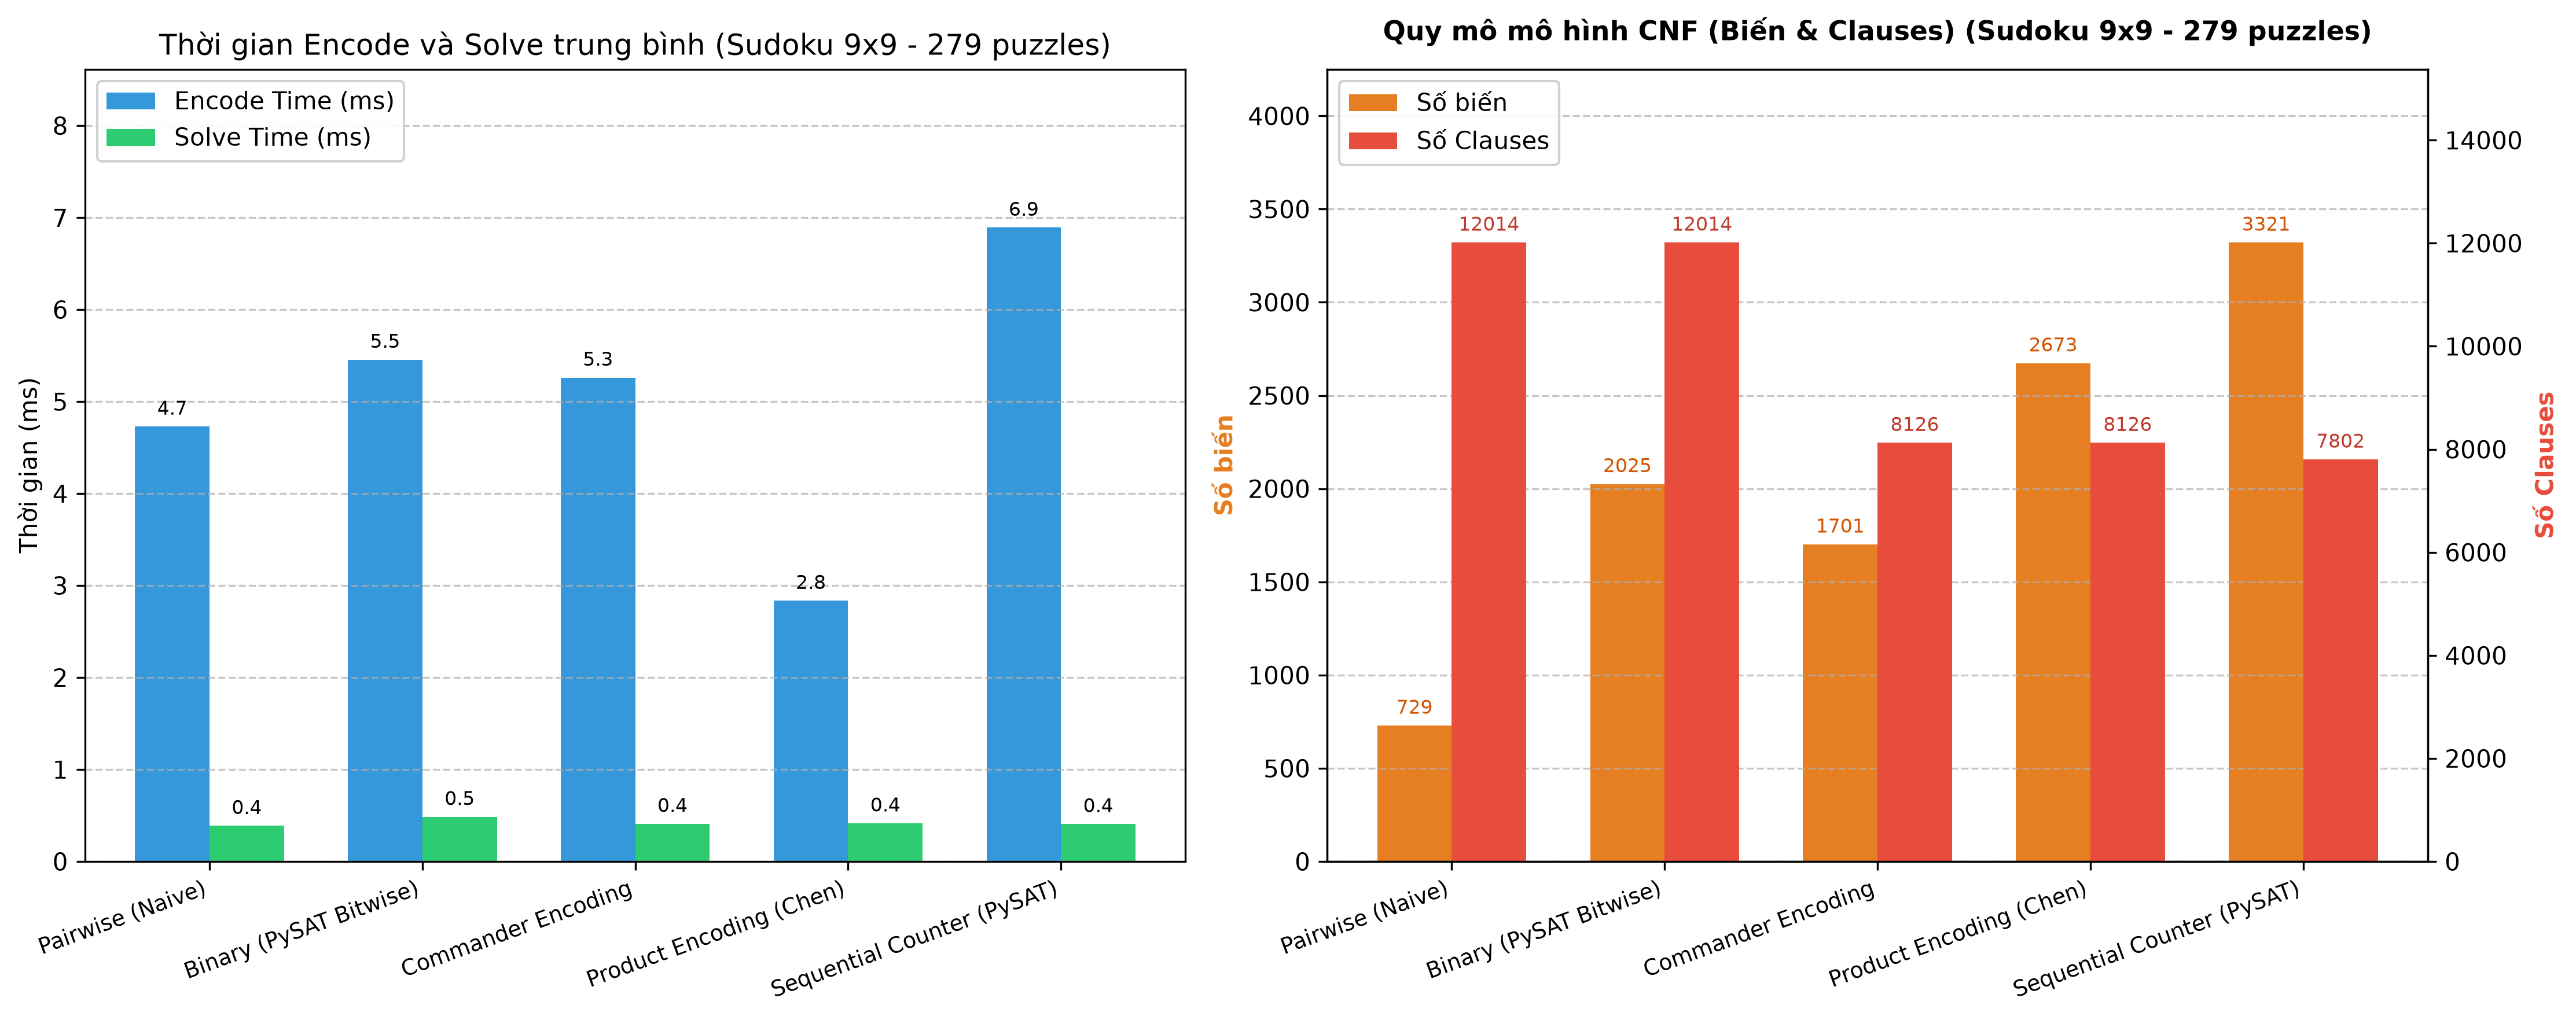
\includegraphics[width=0.92\textwidth]{fig_encodings.png}
\caption{So sánh thời gian Encode vs Solve và quy mô số biến phụ/mệnh đề giữa 5 kỹ thuật SAT Encodings trên tập câu đố chuẩn hóa.}
\label{fig:encodings}
\end{figure*}

\textbf{Phân tích}:
\begin{itemize}
    \item \textit{Về số lượng mệnh đề (Clauses)}: Phương pháp Pairwise có số lượng mệnh đề lớn nhất và bùng nổ theo hàm bậc hai ($12,014$ clauses trên $9\times9$ và vọt lên $123,987$ clauses trên $16\times16$). Ở kích thước $9\times9$, Binary cho số mệnh đề đúng bằng Pairwise do $\binom{9}{2}=36 = 9\lceil\log_2 9\rceil$; tuy nhiên khi $N$ tăng lên $16$, ưu thế tiệm cận $O(n\log n)$ của Binary thể hiện rõ và số mệnh đề giảm còn $66,643$ (khoảng $-46\%$). Các kỹ thuật tuyến tính Commander, 2-Product và Sequential Counter giảm mạnh hơn nữa, khoảng \textbf{32--35\%} trên $9\times9$ và \textbf{58--63\%} trên $16\times16$ so với Pairwise, kiểm soát chặt chẽ hiện tượng bùng nổ mệnh đề khi $N$ tăng.
    \item \textit{Về thời gian mã hóa và giải SAT}: Thời gian mã hóa CNF dao động từ $2.8\text{ ms}$ đến $6.9\text{ ms}$, trong đó \textbf{2-Product} nhanh nhất; còn thời gian giải trên Glucose3 cực kỳ ngắn, chỉ từ $0.4\text{ ms}$ đến $0.5\text{ ms}$ cho mọi phương pháp nhờ cơ chế lan truyền đơn vị. So với thời gian giải, chi phí mã hóa chiếm phần lớn tổng thời gian, vì vậy các kỹ thuật có cấu trúc tuyến tính (tiêu biểu là 2-Product) mang lại tổng thời gian xử lý nhỏ nhất.
\end{itemize}

\subsection{Phân tích độ nhạy cảm theo cấp độ khó (Difficulty Analysis)}
Hình \ref{fig:difficulty} biểu diễn tổng thời gian (mã hóa + giải) trung bình của 5 phương pháp SAT Encoding qua 4 cấp độ khó: \textit{Easy $\to$ Medium $\to$ Hard $\to$ Expert}.

\begin{figure}[t]
\centering
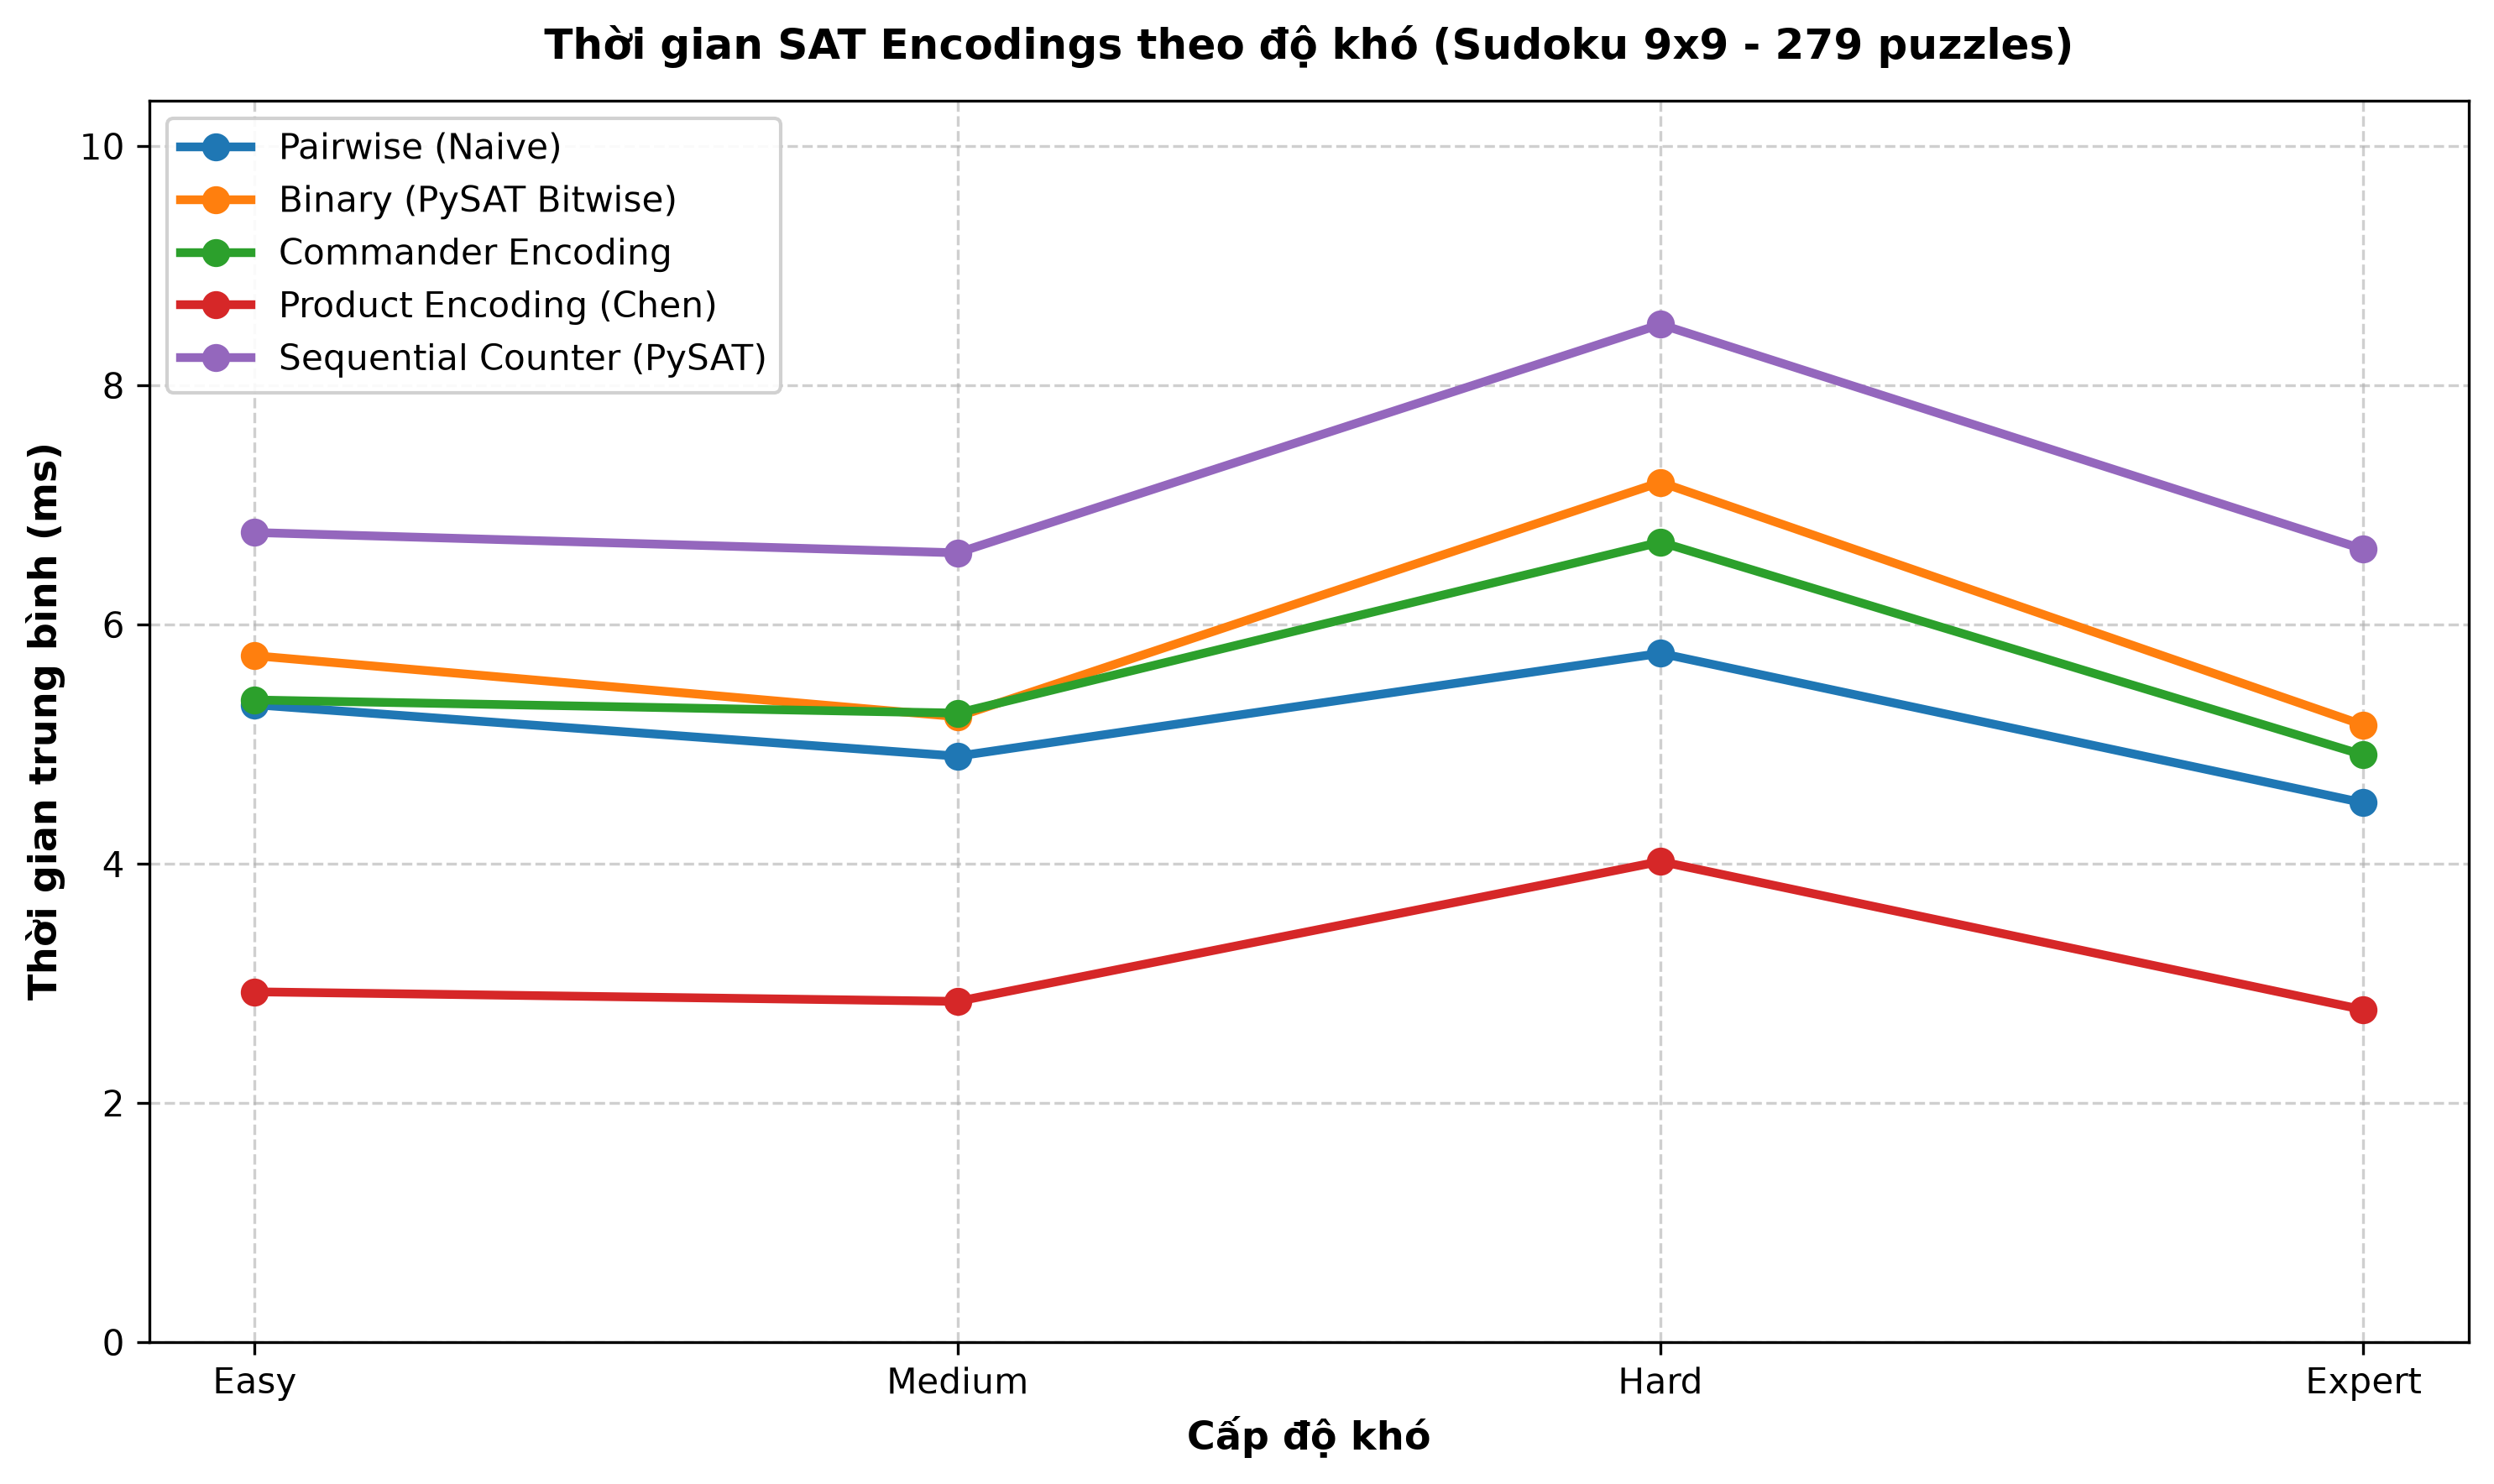
\includegraphics[width=0.85\linewidth]{fig_difficulty.png}
\caption{Xu hướng biến thiên tổng thời gian (mã hóa + giải) của 5 kỹ thuật SAT Encoding theo các cấp độ khó (Sudoku 9x9).}
\label{fig:difficulty}
\end{figure}

\textbf{Nhận xét}:
\begin{itemize}
    \item \textbf{2-Product} là phương pháp ổn định và nhanh nhất ở \textit{mọi} cấp độ khó, dao động khoảng $2.8$--$4.1\text{ ms}$, nhờ chi phí mã hóa thấp nhất và chỉ sinh thêm $2\lceil\sqrt{n}\rceil$ biến phụ.
    \item \textbf{Sequential Counter} có tổng thời gian cao nhất (khoảng $6.5$--$8.6\text{ ms}$) vì phải sinh $n-1$ biến đếm cho mỗi ràng buộc Exactly-One, khiến pha mã hóa trở thành nút cổ chai, dù số mệnh đề sinh ra lại ít nhất.
    \item Thời gian đạt đỉnh tại cấp độ \textit{Hard} rồi giảm nhẹ ở \textit{Expert}; biên độ biến thiên giữa các cấp độ chỉ khoảng $2$--$3\text{ ms}$ và không xuất hiện hiện tượng bùng nổ thời gian (runaway runtime). Điều này cho thấy số lượng gợi ý ban đầu ảnh hưởng không đáng kể tới chi phí xử lý, phần lớn chênh lệch đến từ dao động của pha mã hóa.
    \item Thời gian giải thuần túy trên Glucose3 gần như là hằng số ($0.4$--$0.5\text{ ms}$) cho mọi cấp độ, minh chứng cho hiệu quả của cơ chế lan truyền đơn vị trong các encoding tuyến tính.
\end{itemize}

\subsection{So sánh đối chuẩn hiệu năng giữa SAT Solver và các Solvers (CP, ILP/MIP)}
Bảng \ref{tab:solver_benchmark} và Hình \ref{fig:solvers} minh họa kết quả đo lường thời gian thực thi trung bình giữa các công cụ giải khác nhau trên cùng tập dữ liệu chuẩn hóa.

\begin{table}[t]
\centering
\caption{So sánh thời gian giải trung bình giữa các Solver trên tập 279 câu đố Sudoku $9 \times 9$ chuẩn hóa.}
\label{tab:solver_benchmark}
\begin{tabular}{lccc}
\toprule
\textbf{Bộ giải (Solver Engine)} & \textbf{Trường phái} & \textbf{Thời gian TB (ms)} & \textbf{Tỷ lệ thành công} \\
\midrule
SAT (Glucose3 - Commander) & SAT & \textbf{10.67} & 100\% \\
SAT (Glucose3 - Product) & SAT & \textbf{10.90} & 100\% \\
SAT (Glucose3 - SeqCounter) & SAT & \textbf{11.94} & 100\% \\
SAT (Glucose3 - Pairwise) & SAT & \textbf{13.21} & 100\% \\
SAT (Glucose3 - Binary) & SAT & \textbf{16.91} & 100\% \\
Gurobi Optimizer & MIP & 17.38 & 100\% \\
Google OR-Tools CP-SAT & CP / SAT Hybrid & 19.01 & 100\% \\
IBM CPLEX MIP & MIP & 25.50 & 100\% \\
IBM CPLEX CP Optimizer & CP & 44.73 & 100\% \\
ILP (PuLP / CBC) & ILP / Branch-and-Cut & 147.10 & 100\% \\
\bottomrule
\end{tabular}
\end{table}

\begin{figure}[t]
\centering
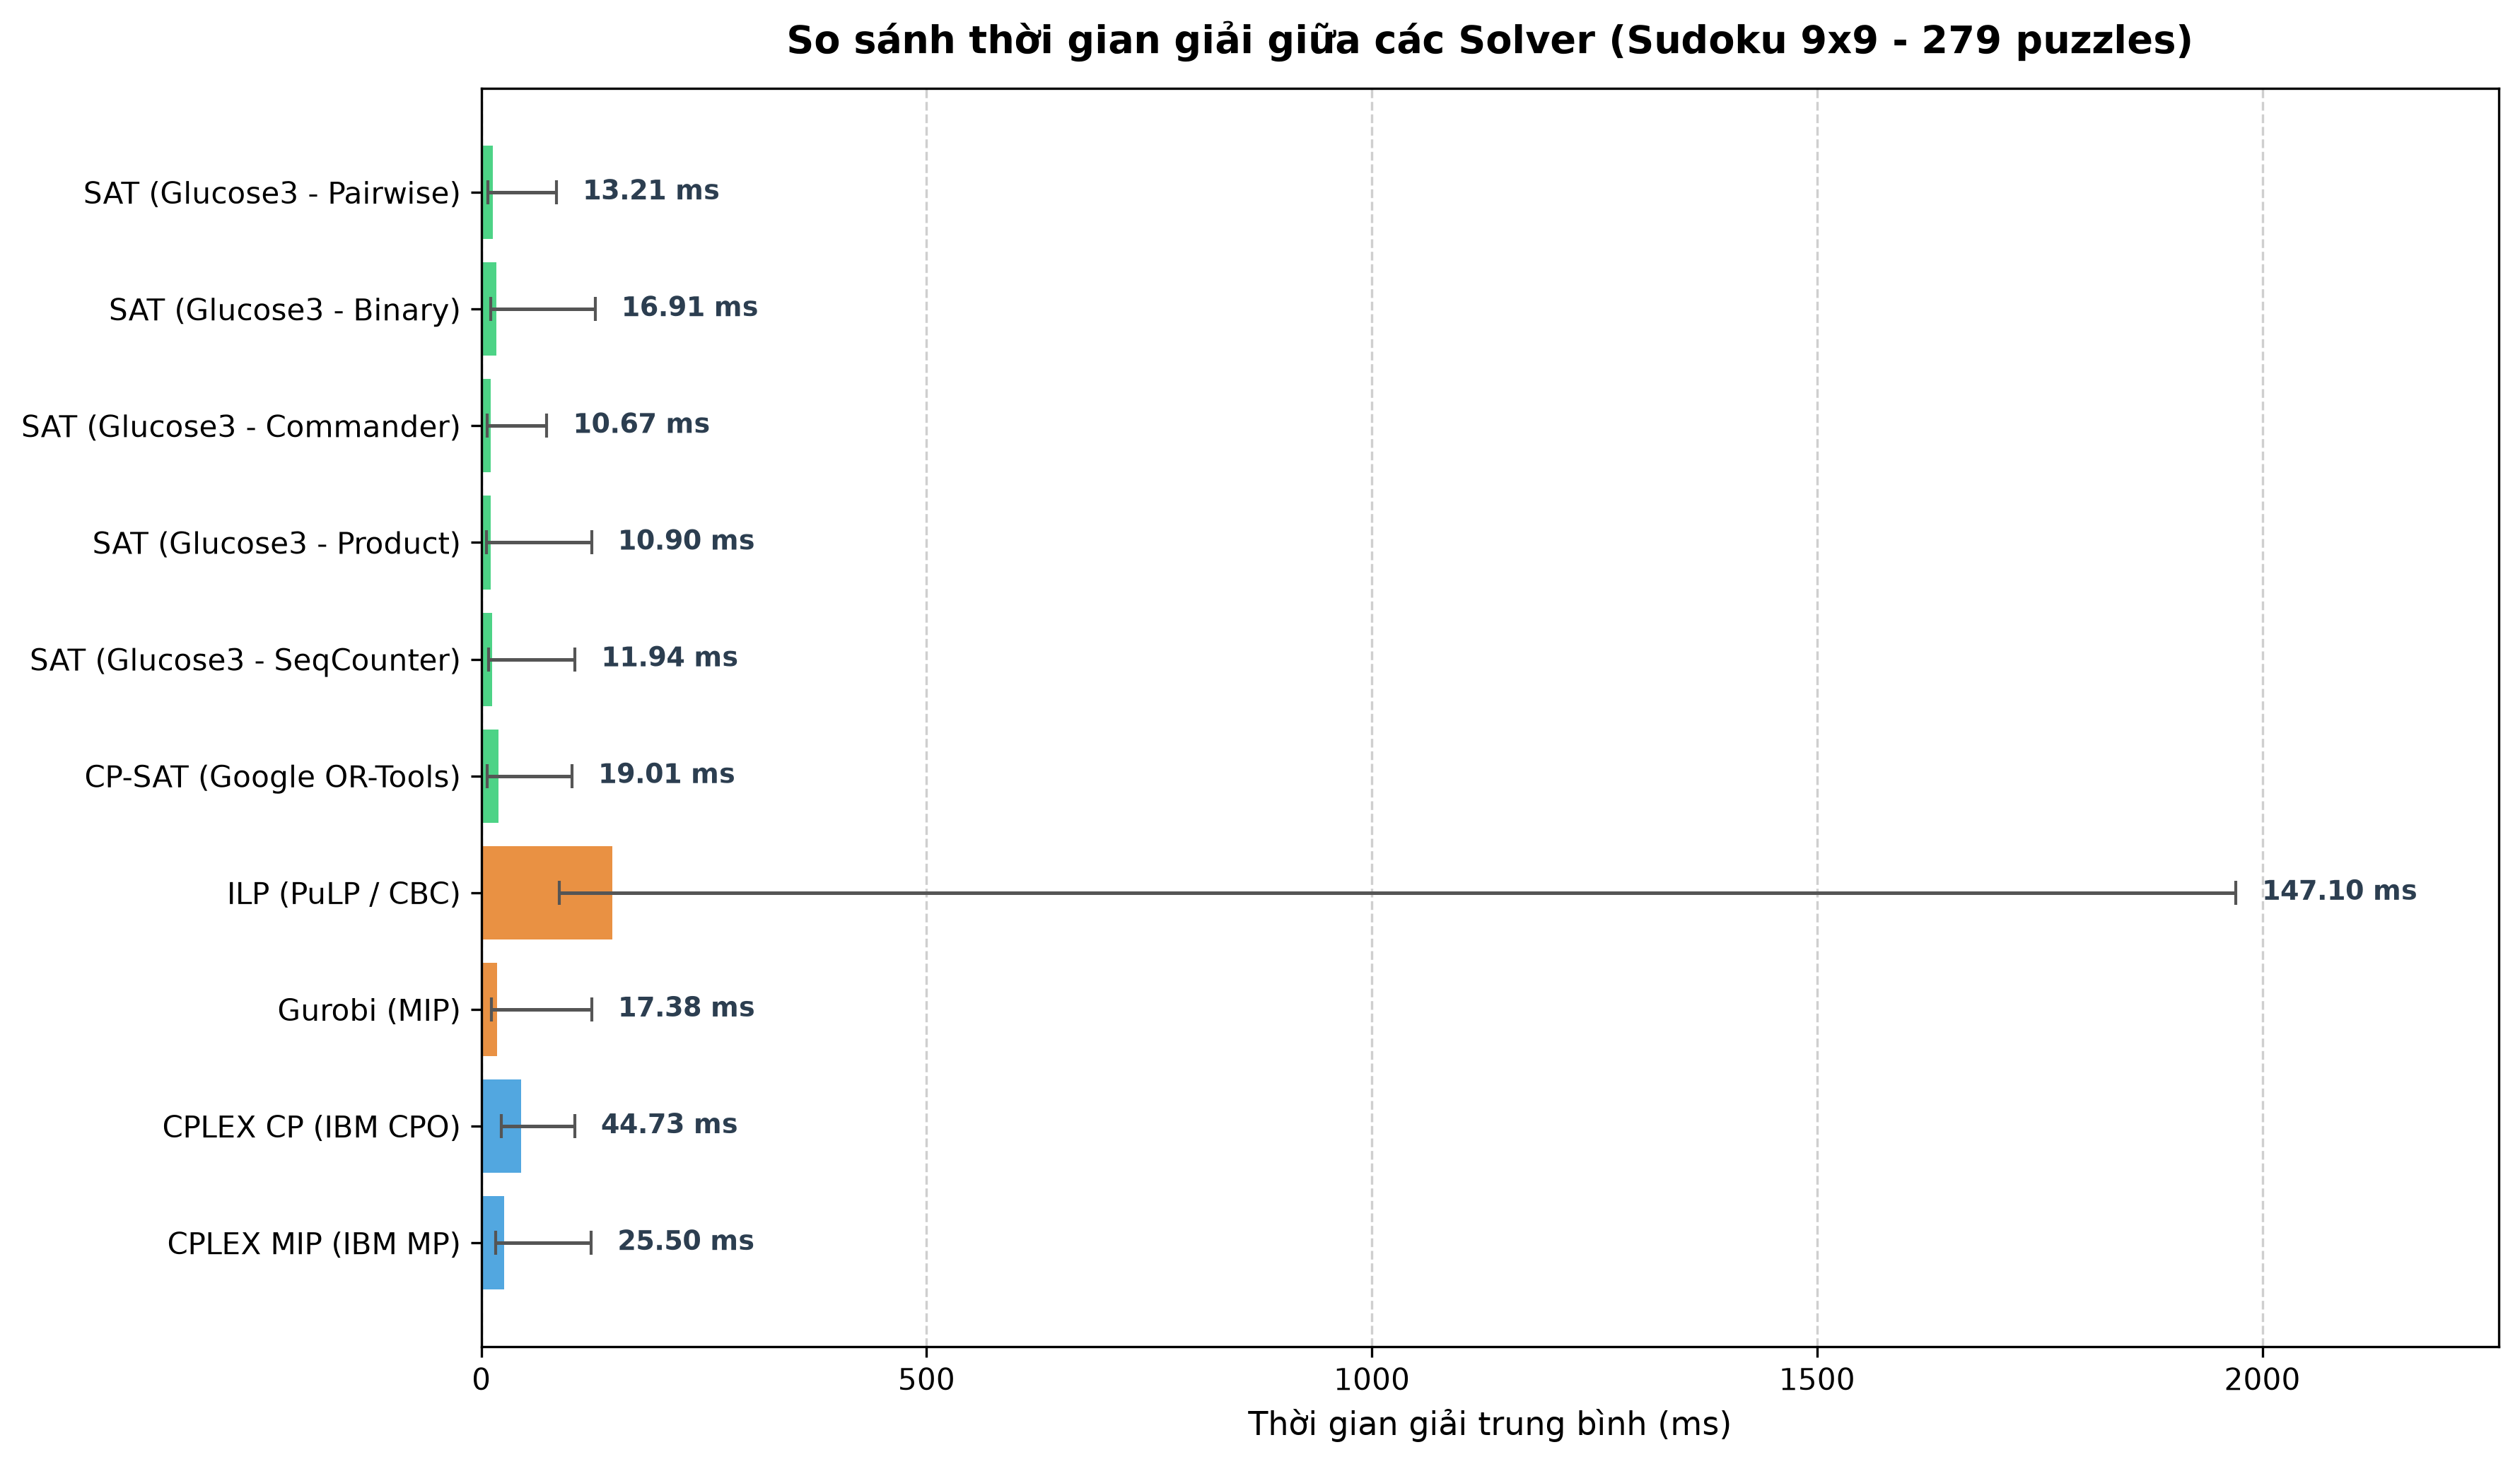
\includegraphics[width=0.88\linewidth]{fig_solvers.png}
\caption{Biểu đồ đối chuẩn thời gian giải giữa SAT Solver (Glucose3) và các bộ giải CP, MIP hàng đầu.}
\label{fig:solvers}
\end{figure}

\textbf{Thảo luận chuyên sâu}:
\begin{enumerate}
    \item \textbf{SAT Solver dẫn đầu về tốc độ}: Với thời gian trung bình $10.7$--$16.9\text{ ms}$ (trung bình khoảng $12.7\text{ ms}$), xét theo encoding SAT nhanh nhất ($10.67\text{ ms}$), SAT Solver (Glucose3) nhanh hơn Gurobi MIP ($17.38\text{ ms}$) khoảng \textbf{1.6 lần}, nhanh hơn CPLEX MIP ($25.50\text{ ms}$) khoảng \textbf{2.4 lần}, nhanh hơn CPLEX CP Optimizer ($44.73\text{ ms}$) khoảng \textbf{4.2 lần} và nhanh hơn solver mã nguồn mở CBC ($147.10\text{ ms}$) tới khoảng \textbf{13.8 lần}. Lý do cốt lõi là bản chất rời rạc thuần túy của Sudoku rất tương thích với cấu trúc biểu diễn nhị phân của SAT cùng cơ chế 2-watched literals của các solver CDCL.
    \item \textbf{Hiệu năng của CP-SAT (Google OR-Tools)}: CP-SAT khá gần với SAT thuần ($19.01\text{ ms}$), chỉ chậm hơn khoảng $1.5$ lần so với SAT nhanh nhất. Điều này hợp lý về mặt lý thuyết vì kiến trúc bên dưới của CP-SAT thực chất là một bộ giải SAT CDCL được mở rộng để hỗ trợ các biến nguyên và bộ lọc lan truyền ràng buộc.
    \item \textbf{Vị thế của Gurobi (MIP)}: Gurobi cho kết quả rất cạnh tranh ($17.38\text{ ms}$), gần bằng các encoding SAT chậm hơn, cho thấy các bộ giải MIP thương mại đã tối ưu rất tốt cho lớp bài toán ràng buộc chặt này.
    \item \textbf{Hạn chế của các bộ giải thuần ILP/MIP}: Các bộ giải MIP xử lý bài toán thông qua việc giải bài toán nới lỏng quy hoạch tuyến tính liên tục (LP Relaxation) bằng phương pháp Simplex hoặc Điểm trong (Interior Point) trước khi cắt nhánh nguyên. Trong bài toán Sudoku, ma trận ràng buộc không đạt tính đơn mô-đun toàn phần (unimodular), nên nghiệm LP nới lỏng thường mang giá trị phân số và cây tìm kiếm phân nhánh bị phình to hơn so với suy diễn logic trực tiếp của SAT. Đây là nguyên nhân chính khiến CBC ($147.10\text{ ms}$) chậm hơn hẳn một bậc độ lớn.
\end{enumerate}

\section{Kết luận và Hướng phát triển (Conclusion)}
Bài báo đã hoàn thành nghiên cứu toàn diện về việc mô hình hóa logic và giải bài toán Sudoku tổng quát $N \times N$ bằng SAT Encoding và đối chuẩn với các công cụ CP/MIP:
\begin{itemize}
    \item Triển khai hoàn chỉnh 5 kỹ thuật mã hóa ràng buộc số lượng At-Most-One: Pairwise, Binary, Commander, 2-Product, và Sequential Counter.
    \item Chứng minh thực nghiệm rằng \textbf{2-Product Encoding} đạt sự cân bằng tốt nhất giữa số biến phụ ($O(\sqrt{n})$), số mệnh đề sinh ra và tổng thời gian xử lý ($2.8$--$4.1\text{ ms}$ trên mọi cấp độ khó); trong khi \textbf{Sequential Counter} sinh ít mệnh đề nhất nhưng tốn nhiều biến phụ và thời gian mã hóa nhất.
    \item Khẳng định lợi thế về tốc độ của tiếp cận \textbf{SAT Solving} đối với lớp bài toán logic tổ hợp hữu hạn so với các bộ giải tối ưu hóa toán học truyền thống (ILP/MIP), dù các bộ giải MIP thương mại (Gurobi) đã bám sát khoảng cách rất nhỏ.
\end{itemize}

\textbf{Hướng phát triển trong tương lai}: Nghiên cứu mở rộng sang các biến thể Sudoku phức tạp hơn (như Killer Sudoku, Diagonal Sudoku, Greater-Than Sudoku) đòi hỏi kết hợp kỹ thuật thỏa mãn modulo lý thuyết (SMT - Satisfiability Modulo Theories) và tối ưu hóa thỏa mãn lớn nhất (MaxSAT).

\section*{Data Availability (Tính sẵn sàng của dữ liệu)}
Toàn bộ mã nguồn chương trình, bộ dữ liệu 299 câu đố benchmark chuẩn hóa, các script đo lường tự động và hình ảnh biểu đồ thực nghiệm chi tiết được công khai phục vụ cộng đồng học thuật tại GitHub repository:
\begin{center}
\url{https://github.com/nmson8206/Sudoku_prj}
\end{center}

\bibliographystyle{cas-model2-names}
\bibliography{references}

\end{document}
